%% This file is automatically generated. Do not edit!
%\documentclass[11pt]{segabs}

%\usepackage{amsmath}
%\usepackage{setspace}
%\usepackage{wasysym}
%\usepackage{graphicx}


%\newcommand{\mb}{\mathbf}
%\DeclareMathAlphabet{\mathcal}{OMS}{cmsy}{m}{n}
%\newcommand{\bv}{\mathbf{v}}
%\newcommand{\bx}{\mathbf{x}}
%\newtheorem{exmp}{Example}


%\setfigdir{Fig}

%\begin{document}
\title{Waveform Inversion via Source Extension}
\author{Guanghui Huang, Michigan State University, Rami Nammour, Total $E\&P$ $R\&T$ USA, William W. Symes, Rice University, Mohamed Dolliazal, Total $E\&P$ $R\&T$ USA}

%\extrafloats{100}

\lefthead{Huang, Nammour, and Symes}

\righthead{Source Extension}

\maketitle
\begin{abstract}
Extended modeling is one of a number of modifications suggested to enhance the reliability of iterative Full Waveform Inversion (FWI), by making it less prone to stagnation away from useful model estimates (``cycle skipping''). All extended modeling methods add parameters to wave modeling beyond those suggested by basic wave physics, in some cases entailing substantial computational expense. Source extension methods add parameters to the description of the physical energy source; many of these cost little more computationally than standard FWI. The first purpose of this paper is to present a (necessarily incomplete) taxonomy of proposed source extensions and related inversion methods. The second purpose is to introduce a particular such method, the Surface Source Extension, and give a couple of examples of its use. We will also explain the theoretical justification for some of these methods: for pure transmission (including diving wave) data, a close link to traveltime tomography explains the absence of cycle skipping observed in numerical experiments. No such theoretical link is known to exist in the case of pure reflection data, but some positive numerical results suggest that some source extension methods may ameliorate cycle-skipping in that case as well .
\end{abstract}

\section{Overview}
FWI can be described in terms of a wave operator $L[c]$ depending on an array of space-dependent coefficient fields $c$, a trace sampling operator $P$, and a dynamic wavefield $u$. The components of coefficient fields $c$ describe material parameters (density, elasticity tensor components, attenuation coefficients,...) and depend on spatial position $\bx$. The dynamical field $u$ may be vector-valued and depends on $\bx$ and on time $t$. The trace sampling operator converts $u$ to a a vector of trace gathers indexed by source position $\bx_s$ representing sensor outputs, or ``data'' for short. The basic FWI problem is: given data $d$,  find coefficients $c$ and source space-time fields $f$ (also indexed by $\bx_s$) so that
\begin{equation}
\label{eqn:fwi}
Pu \approx d \mbox{ and } L[c]u = f.
\end{equation}
Sometimes $f$ is also regarded as given, sometimes only some aspects are given (for example, localization at a source point) and others are to be determined as part of the solution. A basic optimization formulation of FWI is the nonlinear least squares problem:
\[
\mbox{choose } c, f \mbox{ to minimize } \|PL[c]^{-1}f -d \|^2
\]
often with some sort of regularization thrown in.

As is well-known, local optimization methods are the only feasible approach given the dimensions of a typical instance of \ref{eqn:fwi}, and those have a tendency to stall at physically uninformative models due to ``cycle-skipping''.

Many modifications of FWI have been proposed to avoid cycle-skipping. One category of such modifications are the extension methods, in which the FWI problem is ``relaxed'' by adding degrees of freedom to the model. Proposed extension methods fall roughly into two categories: medium extensions, in which parameters are added to the coefficients in the wave equation, and source extension, in which parameters are added to the energy source representation. We shall focus on source extension methods here; see \cite{geoprosp:2008} for an overview of medium extensions, also \cite{Herve2017} for more recent developments. Source extensions effectively impose the wave equation as a soft, as opposed to hard, constraint. For sake of argument (and because almost all work so far has assumed it), adopt the isotropic point source as the physical source model: for the data gather at source position $\bx_s$, the source takes the form
\begin{equation}
\label{eqn:ptsrc}
f(\bx,t;\bx_s) = w(t)\delta(\bx-\bx_s).
\end{equation}
Every method explained below can be altered to accommodate more complex physical source models.

Source extension replaces $f(\bx,t;\bx_s)$ with an artificial source $g(\bx,t; \bx_s)$ with more degrees of freedom than merely a single common source wavelet $w(t)$ as in definition \ref{eqn:ptsrc}. Assuming that \ref{eqn:ptsrc} is actually correct physics, these extra degrees of freedom have to be suppressed in the optimal solution, via an {\em annihilator} $A$, an operator acting on extended sources $g$, whose null space is precisely the physical sources (of the form \ref{eqn:ptsrc}). Extended source inversion replaces the FWI objective with a penalty function
\begin{equation}
\label{eqn:esi}
\mbox{choose } c, g \mbox{ to minimize } \|PL[c]^{-1}g -d \|^2 + \alpha^2 \|A[g]\|^2
\end{equation}

The way in which degrees of freedom are introduced, and the choice of annihilator, distinguish the various source extension methods proposed in the literature. In the next few paragraphs we describe some examples.

\subsection{Wavefield Reconstruction Inversion}
\cite[]{LeeuwenHerrmannWRI:13,LeeuwenHerrmann:16,WangYingst:SEG16,Aghamiry:19} Extended source space consists of arbitrary functions of space-time and source position $g(\bx,t;\bx_s)$. Annihilator is difference with actual (known) source: $A[g]=g-f$.
With these choices, WRI takes the form introduced by \cite{WangYingst:SEG16}. The original approach is equivalent: \cite{LeeuwenHerrmann:16} use the dynamic wavefield $u$ as the additional degrees of freedom, and minimize
\[
\|Pu-d\|^2 + \alpha^2 \|L[c]u-f\|^2
\]
Since the wave equation (any reasonable version!) has a unique solution for each right-hand side, replacing $L[c]u$ with $g$ (and $u$ with $L[c]^{-1}g$) turns this original form of WRI into the form \ref{eqn:esi}.
WRI requires storage of, and access to, the full space-time (or space-frequency) field $g$ (or $u$) at each iteration, potentially a 6D field.

\subsection{Space-Time Extension}
\cite[]{HuangSymes:SEG16b,HuangSymes:Geo18a} Differs from WRI by including $f$ in the unknowns, and in choice of annihilator:
\begin{equation}
\label{eqn:msste}
A[g](\bx,t;\bx_s) = |\bx-\bx_s|g(\bx,t;\bx_s).
\end{equation}
This annihilator merely enforces the position constraint on the source, without relying on {\em a priori} knowledge of the source wavelet. In fact, the source wavelet is a by-product of the minimization \ref{eqn:esi}. Also requires storage of the full (potentially 6D) field.

\subsection{Volume Extension}
\cite[]{HuangSymes:SEG16a,HuangSymes:Geo18b} Assumes that source signature deconvolution has been performed, so that the actual wavelet is (a bandlimited version of) $\delta(t)$. The extended source is an {\em exploding reflector}:
\begin{equation}
\label{eqn:msvol}
g(\bx,t;\bx_s) = h(\bx,\bx_s)\delta(t).
\end{equation}
Uses the same annihilator as the Space-Time Extension, but loses the advantage of solving for the source as by-product - the source must be known, so that decon can be carried out prior to inversion.
However, only requires a (3D) spatial storage volume per source position, essentially equivalent to a second (5D) data volume.

%A disadvantage of this approach, for inversion of reflections, is that unlike post-stack migration the actual physical wave velocity is used in modeling, so that the the region in which $h$ must be defined may considerably larger than the ordinary modeling domain - reflection two-way time is effectively modeled by one-way time.

%The volume extension concept is similar to an idea discussed by \cite{}.

\subsection{Surface Extension}
So far as we know, this extension is described for the first time in this paper (however \cite{ZhangGao:08} describe a related idea). Similar to the volume extension, but the source is spread over the source space-time hypersurface $z=z_s$, rather than over space at $t=0$. In the simplest case, where the sources all lie on $z=z_s$, the extended source space consists of functions (distributions) of the form ($\bx=(x,y,z)$)
\begin{equation}
\label{eqn:mssur}
g(\bx,t;\bx_s) = h(x,y,t;x_s,y_s)\delta(z-z_s).
\end{equation}
As for the previous two cases, the annihilator is given by the localization penalty (equation \ref{eqn:msste}). Therefore the source wavelet is a by-product of the inversion, and does not need to be specified {\em a priori}. Like the volume extension, the additional data volume required is on the same order of size as the data. Unlike the volume extension, it does not require a larger-than-physical simulation volume.

\subsection{Source-Receiver Extension}
\cite{HuangSymes:SEG15a} describe the {\em source-receiver extension}: each trace regarded as separate gather, with separate point source waveform. In effect, the source is permitted to depend on receiver position as well:
\begin{equation}
\label{eqn:awi-alt}
g(\bx,t;\bx_r,\bx_s) = w(t;\bx_r,\bx_s)\delta(\bx-\bx_s).
\end{equation}
Since the corresponding dynamical field $u$ (also dependent on $\bx_r$) satisfies
\begin{equation}
\label{eqn:awi-green}
u(\bx,t;\bx_r,\bx_s)=w(t;\bx_r,\bx_s) *_{t} G(t;\bx,\bx_s)
\end{equation}
it is not necessary to construct $u$ by solving a $\bx_r,\bx_s$-dependent wave equation, only to construct the $\bx_s$-dependent Green's function $G(\cdot; \cdot,\bx_s)$. Thus the modeling cost per iteration is the same as that of FWI.

This extension seems to have appeared first in unpublished work from the third author's group \cite[]{Song:94c,SoSy:92,SongSymes:94a,SongSymes:94b,Symes:94c}. Various annihilators have been suggested, see also \cite[]{Plessix:00a,Plessix:00, PrattSymes:02,LuoSava:11, Warner:14,Warner:16}. Since the source-receiver dependent wavelet $w(t;\bx_r,\bx_s)$ parametrizes the source (equation \ref{eqn:awi-alt}), the annihilator may be viewed as acting on $w$. One popular choice is including multiplication by $t$, which annihilates $w=\delta(t)$:
\begin{equation}
\label{eqn:awi-ann}
A[w](\bx,t;\bx_r,\bx_s) = t w(t;\bx_r,\bx_s)
\end{equation}
This makes sense if the actual source-receiver independent point source wavelet is known and deconvolved from the data traces, to produce an approximate delta source at zero time lag when the coefficients $c$ include kinematically correct velocities.

\subsection{Adaptive Waveform Inversion}
\cite{Warner:14,Warner:16} presented an extended FWI based on source-receiver extension (``Adaptive Waveform Inversion'', AWI) using the scale-by-$t$ annihilator (equation \ref{eqn:awi-ann}). Rather than use the penalty method \ref{eqn:esi}, Warner and Guatsch effectively force the data fit term to zero, by solving the deconvolution problem  $G(t;\bx_r,\bx_s)*_tw(t;\bx_r,\bx_s) = d(t;\bx_r,\bx_s)$, thus making the estimated source wavelet $w(t;\bx_r,\bx_s)$ a function of the coefficients $c$, and using the annihilator term as the objective (several other works cited above have also made use of this $\alpha \rightarrow 0$ limiting case). Further, Warner and Guatsch normalize the objective with the estimated wavelet $L^2$ norm: choose $c$ to minimize
\begin{equation}
\label{eqn:awi-obj}
\sum_{\bx_r,\bx_s}\frac{\int dt\,|t|^2 |w(t;\bx_r,\bx_s)|^2}{\int dt\,|w(t;\bx_r,\bx_s)|^2}
\end{equation}
Note the order of summation and normalization: each trace is normalized independently. This normalization avoids the familiar source/reflector amplitude ambiguity, and has other constructive effects as well.

\section{Theory}
For several of the source extension algorithms, applied to transmission data, the objective is known to be closely linked to traveltime tomography in one form or another, and to inherit its convergence properties. This connection seems first to have been established for the source-receiver extension by \cite{Song:94c} in the case of a so-called differential semblance annihilator, and in \cite[]{HuangSymes:SEG15a,HuangSymes:Geo17} for the time-delay annihilator \ref{eqn:awi-ann}. The latter references study source-receiver extension of constant density acoustic modeling, so that the coefficients $c$ consist of the compressional wave velocity only. As in previous paragraph, make $w$ depend on $c$ by solving the deconvolution problem $G*_tw = d$, then update $c$ to minimize the objective
\begin{equation}
\label{eqn:sr-obj}
 J_0[c,d]= \sum_{\bx_r,\bx_s}\int dt\,|t|^2 |w(t;\bx_r,\bx_s)|^2
\end{equation}
(note that this objective differs from the AWI objective \ref{eqn:awi-obj} by absence of normalization). Assume that the candidate velocity fields are smooth (that is, have no embedded reflectors) and that ray paths connecting sources and receivers are unique. Then for each such velocity $c$, the corresponding Green's function has the asymptotic expansion 
\begin{equation}\label{eqn:green}
G[c](t;\bx_s,\bx_r) = a[c](\bx_s,\bx_r)\delta(t-\tau[c](\bx_r,\bx_s))+R[c](t;\bx_r,\bx_s),
\end{equation}
in which $\tau(\bx_r,\bx_s)$ is the (unique) ray travel time from $\bx_s$ to $\bx_r$ and $a$ is the corresponding geometric amplitude. The remainder $R[c]$ has a Heaviside-type singularity on the light cone $t=\tau(\bx_s,\bx_r) $ and is otherwise smooth \cite[]{Friedlander:75} Choose a target velocity field $c_*$ and create a parametrized family of noise-free data $d_{\lambda}=w_{\lambda}*G[c_*]$ defined by a family of  pulses $w_{\lambda}(t) =\lambda^{-1/2} w_1(t/\lambda) $: the parameter $\lambda$ is effectively the dominant wavelength in the pulse. \cite{HuangSymes:SEG15a} show that under these circumstances,
\begin{equation}
\label{eqn:sr-asympt}
J_0[c,d] \propto \sum_{\bx_r,\bx_s} |\tau[c](\bx_r,\bx_s)-\tau[c_*](\bx_r,\bx_s)|^2 +O(\lambda).
\end{equation}
That is, the objective $J_0$ is proportional to the standard objective function of traveltime tomography, up to an error on the order of dominant wavelength. The same is true of its gradient and Hessian, so the any minimizer of $J_0$ differs from a traveltime tomography solution by an error proportional to wavelength. This fact accounts for the apparent success of source-receiver extension FWI, reported in the cited references.

Unfortunately, the relation between source-receiver extension FWI and traveltime tomography collapses when the rays connecting source and receiver fail to be unique, as occurs generically when velocity field are sufficiently heterogeneous \cite[]{Whi:82}. \cite{Symes:94c} explained this failure and illustrated it numerically. \cite{HuangSymes:Geo17} give a different perspective on the theory, and an explicit illustration in a diving wave setting: if the diving ray field is triplicated, source-receiver extension FWI is just as prone to ``cycle skipping'' as is ordinary FWI.

The volume and surface source extensions in transmission mode are also closely related to traveltime tomography, in the specific guise of {\em slope tomography} or {\em stereotomography}, which has been developed mostly for migration velocity analysis (see \cite{Prieux:13} and references cited there). In contrast with the source-receiver extension, this relationship continues to hold in the presence of multiple ray paths connecting sources and receivers, and explains the success of surface- and volume-extended FWI. Numerical illustrations of this feature can be found in \cite[]{HuangSymes:Geo18b} and in the numerical results section below.

Insofar as the authors are aware, almost nothing is known about why either WRI or the space-time extended FWI converge, or when. Nothing appears to be known theoretically about the behaviour of any of these methods for reflection data, and numerical evidence is ambiguous (see second example below).

\section{Numerical Examples}
We provide two 2D numerical examples of surface-source extended FWI. The first is based on pure transmission data, and illustrates the capability of this extended inversion method to resolve velocities in the presence of multiple ray paths connecting sources and receivers. The second is based on the Marmousi model \cite[]{BoLaVe:91}, modified to ensure that almost all of the recorded energy consists of reflections. Its success underlines a gap in the current theory.

In both examples, modeling and inversion computations are carried out in the frequency domain with standard finite difference stencils and direct matrix methods. The penalty parameter $\alpha$ is set so that the initial data residual in the surface source extended inversion is roughly half the initial data residual for FWI, and held constant throughout the inversion. This resulted in the choices $\alpha=0.001$ for the first (lens) example, $\alpha=1.0$ for the second (Marmousi) example. We also added a regularization term, a multiple of the mean square gradient of the velocity field, weighted to be initially 10\% of the sum of the data and penalty terms, as in our work on the volume source extension \cite[]{HuangSymes:Geo18b}. We used the LBFGS algorithm \cite[]{NocedalWright} to perform all inversions.

{\exmp{(Low velocity zone)}} This example closely resembles one used by \cite{HuangSymes:SEG15a,HuangSymes:Geo18a} to demonstrate the failure of source-receiver extended inversion in the presence of multiple ray paths. The velocity model consists of a Gaussian low velocity anomaly embedded in a constant background model $v_0=2$ km/s (Figure \ref{fig:GaussVt}):
\begin{equation}
    v(x,z) = 2 - 1.4e^{-\frac{(x-1)^2}{0.25^2} -\frac{(z-1)^2}{0.5^2}} km/s.
\end{equation}
Source depth is $z_s=1.99$ km, receiver depth $z_r=0.01$ km.
A shot gather generated with a 10 Hz Ricker wavelet at $x_s=1.5$ km appears as Figure \ref{fig:GvData1500m}. Triplicated arrivals due to the low velocity anomaly are clearly evident.

\inputdir{./Fig/gv}

\begin{figure}[h]
 \centering
     \subfloat[\label{fig:GaussVt}]{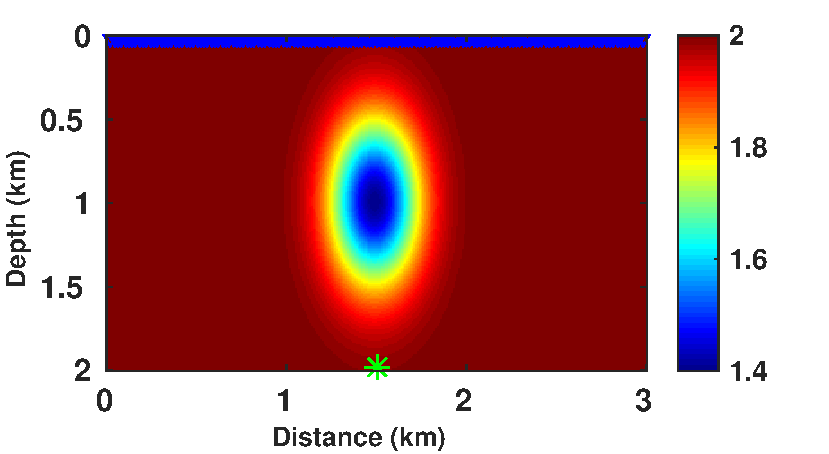
\includegraphics[width=0.5\columnwidth]{Fig/gv/GaussVt}}
     \subfloat[\label{fig:GvData1500m}]{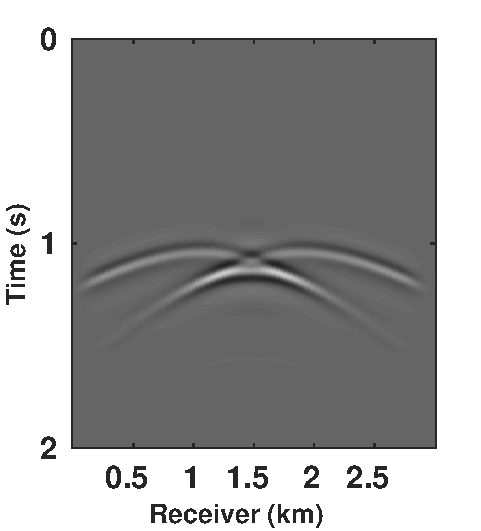
\includegraphics[width=0.245\columnwidth]{Fig/gv/GvData1500m}}
     \caption{Transmission problem: (a) Gaussian low velocity anomaly model and (b) recorded data. Receivers (blue star) and sources (green star) are placed on the top and bottom to mimic the transmission configuration.}
\end{figure}


%\multiplot{2}{,GvData1500mV0}{width=0.3\columnwidth}{Transmission problem: Shot gather of (a) recorded data and (b) simulated data by constant velocity $v_0$ for shot at $x_s=1.5$ km. Due to the low velocity anomaly, complicated triplications are present in the recorded data, and arrive later than the event by constant velocity.}

%\multiplot{3}{GaussV0pt8,GaussV0pt8,GaussVt}{width=0.3\textwidth}{Transmission problem: (a) constant velocity ($v_0$), (b) testing velocity $v = 0.8v_t+0.2v_0$ and (c) true velocty $v_t$.}

%\multiplot{3}{GvBackpro1500m,GvExtSrc1500m,GvExtData1500m,GvV0pt8Backpro1500m,GvV0pt8ExtSrc1500m,GvV0pt8ExtData1500m,GvVtBackpro1500m,GvVtExtSrc1500m,GvVtExtData1500m}{width=0.27\columnwidth}{Transmission problem: (a) backpropagation wavefield of recorded data at $x_s=1.5$ km, (b) extended source model and (c) extended data by constant velocity $v_0$; (d)-(f) are similar plots as the top row but computed by testing velocity $v=0.8v_t+0.2v_0$; (g)-(i) are similar plots as the top row but computed by true velocity $v_t$;  }


\begin{figure}[h]
 \centering
     \subfloat[\label{fig:GaussV31its}]{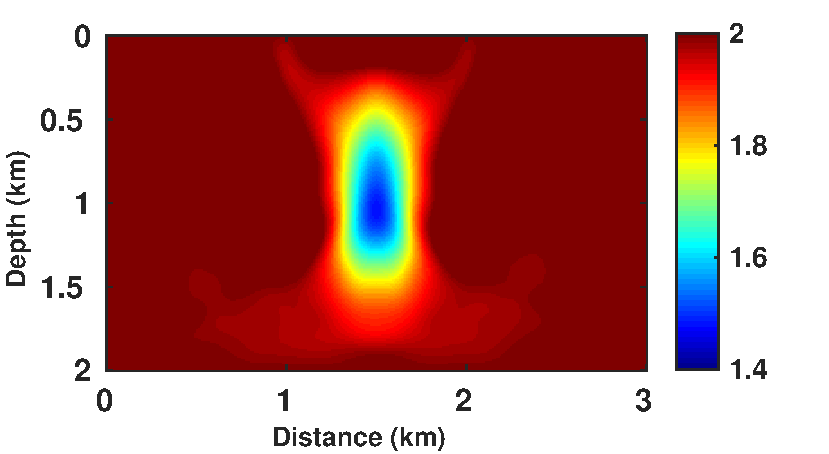
\includegraphics[width=0.5\columnwidth]{Fig/gv/GaussV31its}}
\subfloat[\label{fig:GvExtSrc1500m}]{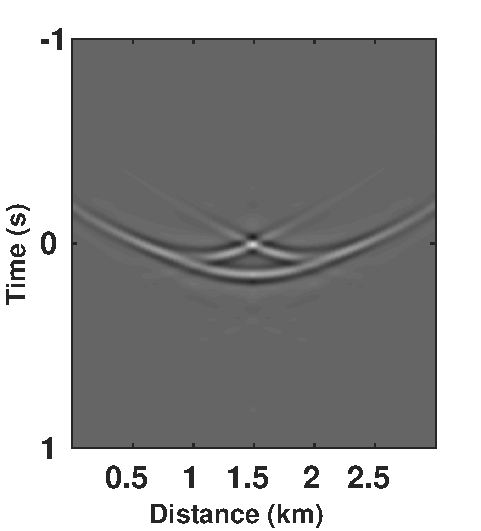
\includegraphics[width=0.245\columnwidth]{Fig/gv/GvExtSrc1500m}}
     \subfloat[\label{fig:GvV31its10HzExtSrc1500m}]{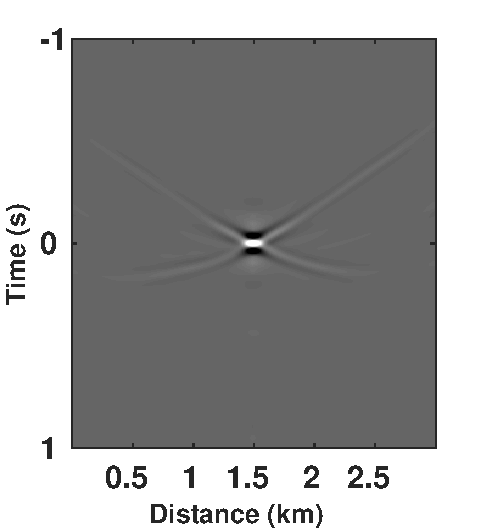
\includegraphics[width=0.245\columnwidth]{Fig/gv/GvV31its10HzExtSrc1500m}}
     \caption{Transmission problem: (a) inverted velocity by surface source extended FWI; (b) extended source estimate using initial constant velocity; (c) extended source estimate using the final inverted velocity. Both (b) and (c) for shot at $x_s=1.5$ km.}
\end{figure}
After 31 LBFGS iterations, the surface source extended FWI algorithm obtains the velocity estimate depicted in Figure \ref{fig:GaussV31its}.  Source energy is much more focused in time and space after inversion (Figures \ref{fig:GvExtSrc1500m}, \ref{fig:GvV31its10HzExtSrc1500m}).

{\exmp{(Marmousi)}}
We modified the Marmousi model by adding a $2.2$ km water layer and truncating the depth range at $4$ km, also adding a box-like high velocity anomaly at $z=$2.2 km, $x=$2.8 km in distance (Figure \ref{fig:Marm2kmVt}). Grid increments were $\Delta x = \Delta z = 0.02$ km. The 2.2 km deep water effectively gates out refraction (diving) waves, so that the data energy is almost purely reflection. We generated 8 s of data for a fixed receiver spread using an isotropic point source with 8 Hz Ricker wavelet, receiver coordinates $z_r=0.04$, $x_r=$ 0.05 km to 9.15 km, $\Delta x_r=$ 0.05 km, source coordinates $z_s=0.08$ km, $x_s=0.6$ km to $x_s=8.6$, $\Delta x_s$ = 0.1 km. Figures \ref{fig:Marm2kmShot1}-\ref{fig:Marm2kmShot81} show shot gathers at $x_s=0.6$ km and $x_s=8.6$ km.

The initial velocity (Figure \ref{fig:Marm2kmV0}) is linearly increasing with depth below the water layer. Data for both FWI and surface source extended FWI, method are sampled from the Fourier-transformed time domain traces with frequency band [5,8] Hz. The correct source amplitudes were input for FWI, whereas the surface source extended FWI generates these as by-product.

\inputdir{./Fig/marm2km}

\plot{Marm2kmVt}{width=0.8\columnwidth}{Marmousi example: the modified Marmousi model added with 2.2 km  water layer on the top and a high velocity salt box around the left part of the model. The water layer of 2.2 km in depth is used to avoid the refraction energy present in the recorded data.}

\multiplot{1}{Marm2kmV0,Marm2kmFWI,Marm2kmSurf}{width=0.8\columnwidth}{Marmousi example: (a) 1D initial velocity; inverted results by (b) FWI  with target source wavelet and (c) by surface source based MSWI without given source wavelet.}

\multiplot{2}{Marm2kmShot1,Marm2kmShot81}{width=0.4\columnwidth}{Marmousi example: shot gather of recorded data for shot at (a) $x_s=0.6$ km and (b) $x_s=8.6$ km.}

\multiplot{2}{Marm2kmShot1Inv,Marm2kmShot81Inv}{width=0.4\columnwidth}{Marmousi example: shot gather of  simulated data generated using the inverted velocity by surface source based MSWI for shot at (a) $x_s=0.6$ km and (b) $x_s=8.6$ km..}



The 200th FWI iterate is shown in Figure \ref{fig:Marm2kmFWI}, the 150th surface source extended FWI iterate in Figure \ref{fig:Marm2kmSurf}. All features of the target model, at both large and small scales to the resolution afforded by the data, are much better imaged in the latter.  Figures \ref{fig:Marm2kmShot1Inv}-\ref{fig:Marm2kmShot81Inv} show the simulated  data produced by the final inverted velocity, which compare very well with the target data (Figures \ref{fig:Marm2kmShot1}, \ref{fig:Marm2kmShot81}).

\section{Conclusion}
We have described the source extension modification of FWI, detailed several methods of this type found in the literature, and used the surface source extension to illustrate the type of result obtainable using this class of FWI modifications. Theoretical understanding is currently limited to transmission data inversion: several of the extended source FWI algorithms are closely related to variants of travel time tomography, and produce results of similar quality. No theoretical results are available for reflection data, nor for several source extensions described in the literature, notably WRI. Also, several promising algorithms are numerically challenging, requiring data storage and/or computation far in excess of the norm for conventional FWI. Both theory and algorithm development are promising avenues for further research on extended source FWI.

\paragraph{Acknowledgement:} GH and WS thank The Rice Inversion Project and Total E\&P USA for support. We thank Total E\&P USA for permission to publish these results.

\bibliographystyle{seg}
\bibliography{../../bib/masterref}
%\bibliography{masterref}
%\end{document}
